\documentclass[12pt, letterpaper]{article}
\usepackage{graphicx} % Required for inserting images

\usepackage[
    top=5mm,
    bottom=5mm,
    left=5mm,
    right=5mm,
    marginparwidth=0mm,
    marginparsep=0mm,
    headheight=15pt,
    headsep=0pt,
    centering,
    % showframe,
    includehead
    ]{geometry}

\usepackage{setspace}
\usepackage{titlesec}
\usepackage{lipsum}
\usepackage{amsmath}
\usepackage{enumitem}

\usepackage{blindtext}
\usepackage{multicol}
\usepackage{fancyhdr}
\usepackage{tikz}

\usetikzlibrary{fit}

% load the preamble
\input{preamble/preamble}



\newcommand{\blue}[1]{
\color{blue} #1 \color{black}
}

\newcommand{\red}[1]{
\color{red} #1 \color{black}
}

\newcommand{\fl}[1]{
    \left\lfloor #1 \right\rfloor
}

\newcommand{\ce}[1]{
    \left\lceil #1 \right\rceil
}

\newcommand{\tr}[2]{
    \left(\frac{#1}{#2}\right)
}



% add more margin between multicols columns
\setlength\columnsep{10pt} 

\vspace{-\baselineskip}


% remove all paragraph indents
\setlength{\parindent}{0pt}

% reduce the spacing in lists
\setlength{\parskip}{1pt}
\setlist{
    noitemsep,
    topsep=0pt,
    partopsep=0pt,
    itemindent=0pt,
    listparindent=0pt,
    leftmargin=15pt%\dimexpr 26pt- 12pt
}

% ================== %
% format of sections
% ================== %
\titleformat{\section}
   {\normalfont\fontsize{8}{12}\bfseries\MakeUppercase}{}{1em}{\underline}
%\titlespacing{\section}{-1pc}{10pt}{1pt}
\titlespacing{\section}{-1pc}{0pt}{0pt}

\titleformat{\subsection}
   {\normalfont\fontsize{8}{10}\bfseries}{}{1em}{}
% \titlespacing{\subsection}{-0.7pc}{1pt}{1pt}
\titlespacing{\subsection}{-1pc}{0pt}{0pt}

\titleformat{\subsubsection}
   {\fontsize{8}{10}\bfseries\sc}{}{1em}{}
% \titlespacing{\subsection}{-0.5pc}{1pt}{1pt}
\titlespacing{\subsubsection}{-1pc}{0pt}{0pt}



% ================= %
% Headers & Footers
% ================= %
\pagestyle{fancy}
\fancyhf{}
\lhead{\underline{\sc CMSC420 Cheatsheet}}
% \rhead{\footnotesize Ga\"etan Almela, Grayson Wolf, Danesh Sivakumar, Mazin Karjikar}
\rfoot{\thepage}
\renewcommand{\headrulewidth}{0pt}



% ================= %
% Aliases
% ================= %
\def\cov{\text{Cov}}
\def\corr{\text{Corr}}
\def\var{\text{V}}
\def\ev{\text{E}}
\def\eps{\varepsilon{}}


% remove page numbers from ToC
\addtocontents{toc}{\protect\thispagestyle{empty}}
\pagenumbering{gobble}



% boxed scope
\pgfmathsetmacro\myscopelevel{0}
\newenvironment{bscope}[0]
{
  \pgfmathsetmacro\myscopelevel{int(\myscopelevel+1)}
  %\typeout{myscopelevel:\myscopelevel}
  \begin{scope}[local bounding box/.expanded=bounding box \myscopelevel]
  }{
  \end{scope}
  \node [draw, inner sep=1pt, dashed, fit=(bounding box \myscopelevel), rectangle] {};
}



% ================= %
% Document
% ================= %
\begin{document}
    \tiny
    \begin{multicols*}{3}

        % UNCOMMENT IF WE WANT TABLE OF CONTENTS?
        % \tableofcontents
        \section{Sum Formulas}

        \begin{enumerate}
            \item $\sum_{i = 1}^{n} 1 = n$
            \item $\sum_{i = 1}^{n} i = \frac{n(n + 1)}{2}$
            \item $\sum_{i = 1}^{n} i^2 = \frac{n(n+1)(2n + 1)}{6}$
            \item $\sum_{i = 0}^{n} r^i = \frac{r^{n + 1} - 1}{r - 1} \text{for $|r| < 1$}$
            \item $\sum_{i = 0}^{n} 2^i = 2^{n + 1} - 1$
            \item $\sum_{i = 0}^{n} i 2^i = (n - 1) 2^{n + 1} + 2$
        \end{enumerate}

    
        \section{Amortized Analysis}

        Things to add?
        \begin{enumerate}
            \item Why do we even do this? The goal is to obtain worst case per-operation cost
            \item Token Method (a.k.a Bankers Method): Reallocation problems.
        \end{enumerate}

        \subsection{Complexity Classes}

        \begin{enumerate}
            \item $o(n)$: $f < g$
            
            $f(n) \in o(g(n))$ if $\lim_{n \to \infty} \frac{f(n)}{g(n)} = 0$
            
            {\it $f$ grows {\bf slower} than $g$}.
            
            \item $\O(n)$: $f \le g$

            $f(n) \in \O(g(n))$ if $\exists C > 0, \exists n_0 \ge 1 \text{ such that } \forall n \ge n_0, f(n) \le Cg(n)$.

            {\it Asymptotic upper bound}.
            
            \item $\Theta(n)$: $f = g$
        
            $f(n) \in \Theta(g(n))$ if $\exists B > 0, C > 0, n_0 \ge 1$ such that $\forall n \ge n_0, Bg(n) \le f(n) \le Cg(n)$
            
            {\it Asymptotic upper and lower bound}.
            
            \item $\Omega(n)$: $f \ge g$
        
            $f(n) \in \Omega(g(n))$ if $\exists B > 0, \exists n_0 \ge 1$ such that $\forall n \ge n_0, f(n) \ge Bg(n)$
            
            {\it Asymptotic lower bound}.
            
            \item $\omega(n)$: $f > g$
        
            $f(n) \in \omega(g(n))$ if $\lim_{n \to \infty} \frac{g(n)}{f(n)} = 0$
            
            {\it $f$ grows {\bf faster} than $g$}.
        \end{enumerate}

        \subsection{Aggregate Method}
        Calculate the worst-case cost of $n$ operations and then divide by $n$.

        \subsection{Token Method}

        Each operation has a cost of $\beta = AC(n)$ tokens. For cheap operations $\beta > 0$,
        for expensive operations, $\beta < 0$. Your goal is to find $\beta$.
        
        For $\{x_1, \dots, x_n\}$ operations, we want $(\beta - x_1) + \cdots + (\beta - x_n) = 0$.

        % \TODO{} This is incomplete and I dont really know how to explain this method very well,
        % because it just seems like a long-winded way of doing the aggregate method.


        % \section{Trees}

        % \TODO{}

        % What Justin said in class about this:

        % We talked about
        
        % \begin{enumerate}
        %     \item Any kind of tree.
        %     \item Definition of Height
        %     \item preorder, inorder, postorder traversals
        %     \item What inorder succ and pred mean
        %     \item Threaded binary trees (wait wtf is that?)
        % \end{enumerate}


        
        % \section{Binary Search Trees}

        % \TODO{}

        % What Justin said in class about this:

        % We talked about
        
        % \begin{enumerate}
        %     \item Definition
        %     \item Search, Insert, Delete (how to do replacements?)
        %     \item Time Complexity for all of them
        %     \item Comments about Tree Height (max size is $n$, could be a linked list, min is $\log n$, avg is $\log n$)
        % \end{enumerate}
        



        
        \section{AVL Trees}
        {\it Balanced Binary Search Trees}.

        \subsection{Height \& Balance Factor}
        \begin{itemize}
            \item For a node $n$ with subtrees $L$ and $R$ we have $b(n) = \texttt{height}(R) - \texttt{height}(L)$
            \item A node $n$ is {\it AVL balanced} if $b(n) \in \{-1, 0, 1\}$. All nodes must be AVL balanced.
            \item Height is $\Theta(\log n)$
            % \item \TODO{} Formulas for min/max heights
        \end{itemize}

        \subsection{Rotations}
        {\it The node being rotated is circled.} $A, B, C,$ and $D$ are subtrees, not nodes.
        
        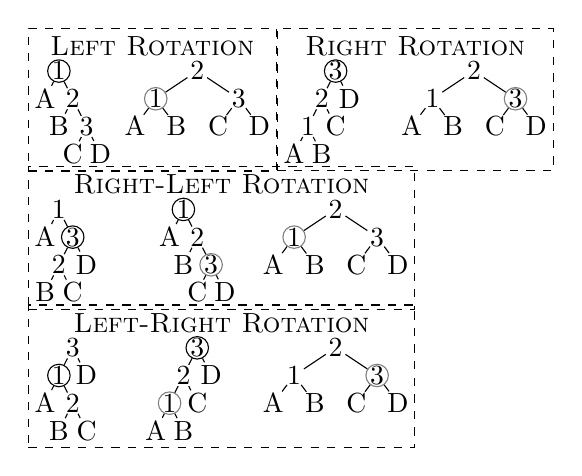
\begin{tikzpicture}[
              level distance= 10pt,
              every node/.style={circle, inner sep=0pt, minimum width=0.25cm}
        ]
            \begin{bscope}
                \begin{scope}[level/.style={sibling distance=10pt}]
                    \node[draw] {1}
                      child {node {A}}
                      child {node {2}
                        child {node {B}}
                        child {node {3}
                            child {node {C}}
                            child {node {D}}
                        }
                      };
                \end{scope}
                
                \begin{scope}[level/.style={sibling distance=30pt/#1}, xshift=50pt]
                    \node {2} 
                      child {node[draw=gray] {1}
                        child {node {A}}
                        child {node {B}}
                      }
                      child {node {3}
                        child {node {C}}
                        child {node {D}}
                      };
                \end{scope}
                \node [yshift=5pt, inner sep=2pt, rectangle] at (bounding box \myscopelevel.north) {\sc Left Rotation};
            \end{bscope}
            
            \begin{scope}[xshift=100pt]
                \begin{bscope}
                    \begin{scope}[level/.style={sibling distance=10pt}]
                        \node[draw] {3}
                          child {node {2}
                            child {node {1}
                                child {node {A}}
                                child {node {B}}
                            }
                            child {node {C}}
                          }
                          child {node {D}};
                    \end{scope}
                    \begin{scope}[level/.style={sibling distance=30pt/#1}, xshift=50pt]
                        \node {2} 
                          child {node {1}
                            child {node {A}}
                            child {node {B}}
                          }
                          child {node[draw=gray] {3}
                            child {node {C}}
                            child {node {D}}
                          };
                    \end{scope}
                    \node [yshift=5pt, inner sep=2pt, rectangle] at (bounding box \myscopelevel.north) {\sc Right Rotation};
                \end{bscope}
            \end{scope}
            
            \begin{scope}[yshift=-50pt]
                \begin{bscope}
                    \begin{scope}[level/.style={sibling distance=10pt}]
                        \node {1}
                          child {node {A}}
                          child {node[draw] {3}
                            child {node {2}
                                child {node {B}}
                                child {node {C}}
                            }
                            child {node {D}}
                          };
                    \end{scope}
                    
                    \begin{scope}[level/.style={sibling distance=10pt}, xshift=45pt]
                        \node[draw] {1}
                          child {node {A}}
                          child {node {2}
                            child {node {B}}
                            child {node[draw=gray] {3}
                                child {node {C}}
                                child {node {D}}
                            }
                          };
                    \end{scope}
                    
                    \begin{scope}[level/.style={sibling distance=30pt/#1}, xshift=100pt]
                        \node {2} 
                          child {node[draw=gray] {1}
                            child {node {A}}
                            child {node {B}}
                          }
                          child {node {3}
                            child {node {C}}
                            child {node {D}}
                          };
                    \end{scope}
                    \node [yshift=5pt, inner sep=2pt, rectangle] at (bounding box \myscopelevel.north) {\sc Right-Left Rotation};
                \end{bscope}
            \end{scope}
            
            \begin{scope}[yshift=-100pt, xshift=5pt]
                \begin{bscope}
                    \begin{scope}[level/.style={sibling distance=10pt}]
                        \node {3}
                          child {node[draw] {1}
                            child {node {A}}
                            child {node {2}
                                child {node {B}}
                                child {node {C}}
                            }
                          }
                          child {node {D}};
                    \end{scope}
                    
                    \begin{scope}[level/.style={sibling distance=10pt}, xshift=45]
                        \node[draw] {3}
                          child {node {2}
                            child {node[draw=gray] {1}
                                child {node {A}}
                                child {node {B}}
                            }
                            child {node {C}}
                          }
                          child {node {D}};
                    \end{scope}
                   
                    \begin{scope}[level/.style={sibling distance=30pt/#1}, xshift=95pt]
                        \node {2} 
                          child {node {1}
                            child {node {A}}
                            child {node {B}}
                          }
                          child {node[draw=gray] {3}
                            child {node {C}}
                            child {node {D}}
                          };
                    \end{scope}
                    \node [yshift=5pt, inner sep=2pt, rectangle] at (bounding box \myscopelevel.north) {\sc Left-Right Rotation};
                \end{bscope}
            \end{scope}
        \end{tikzpicture}        
        % \usegdlibrary{trees}
        % \begin{tikzpicture}
        %     \usetikzlibrary {graphs, graphdrawing} \usegdlibrary {trees}
            
        %     \tikz [baseline=(a.base), tree layout, minimum number of children=2,
        %            sibling distance=5mm, level distance=5mm]
        %       \graph [nodes={circle, inner sep=0pt, minimum size=2mm, fill, as=}]{
        %         a -- { b -- c -- { d -- e, f -- { g, h }}, i -- j -- k[second] }
        %       };\quad
              
        %     \tikz [baseline=(a.base), tree layout, minimum number of children=2,
        %            sibling distance=5mm, level distance=5mm]
        %       \graph [nodes={circle, inner sep=0pt, minimum size=2mm, fill, as=}]{
        %         a -- { b -- c -- d -- e, i -- j -- { f -- {g,h}, k } }
        %       };
        % \end{tikzpicture}

        \subsection{Search}
        Same as BST.
        
        {\bf Worst Case}: $\O(\log n)$

        \subsection{Insert}
        Let $n$ be the node to insert.
        \begin{enumerate}
            \item Insert $n$ as with BST.
            \item Recurse back up tree, looking for any node $n'$ that is not AVL balanced. If found, rotate $n'$ using one of the four rotations.
        \end{enumerate}

        {\bf Worst Case}: $\O(\log n)$


        \subsection{Delete}
        Let $n$ be the node to delete.
        \begin{enumerate}
            \item Replace $n$ with its inorder successor $n'$.
            
            Note: $n'$ now either has only one, or zero subtrees.
            
            \item If $n'$ is a leaf, delete it.
            \item If $n'$ is not a leaf, promote its subtree.
            \item Check if the parent of $n'$ is now unbalanced and fix.
        \end{enumerate}
        
        {\bf Worst Case}: $\O(\log n)$




        
        \section{2-3 Trees}

        \begin{enumerate}
            \item Always perfect.
            \item Height $h \ge -1$, $\O(\log n)$ and $\O(\log k)$.
            \item Empty if and only if $h = -1$.
            \item B-Tree with $m = 3$
        \end{enumerate}

        \subsection{Parameters}
        \begin{enumerate}
            \item $h$: Height of tree.
            \item $k$: Number of nodes.
            \item $k$: Number of keys.
        \end{enumerate}



        \subsection{Search}
        Same as BST.

        { \bf Time Complexity}: $\O(\log n)$.
        
        \subsection{Insert}
        Let $x$ be the key to insert.
        \begin{enumerate}
            \item Follow search path down to a leaf (always).
            \item Add $x$ to leaf.
            \begin{enumerate}[label=\roman*.]
                \item If this does not make the node overfull, done.
                \item Otherwise, promote middle key up, left and right key become two nodes. Push the middle key into the node above. Possibly recurse this process.
            \end{enumerate}
        \end{enumerate}
        % Take a key and follow the search path down to a leaf node, and add it into the leaf node. If this creates a node with three keys, promote the middle key up and treat the left and right keys as its children. This may fuck with the parent, so we possibly have to recurse.

        { \bf Time Complexity}: $\O(\log n)$.
        
        {\bf Don't rotate ever when inserting!} That's how it was invented
        
        \subsection{Delete}
        Do the BST thing until you reach a leaf, then remove the key. If you make a 0-key "hole", fix it like so:
        
        \begin{center}
            \includegraphics[scale=0.1]{23.jpeg}
        \end{center}

        { \bf Time Complexity}: $\O(\log n)$.






        
        \section{B-Trees}
        {\it Generalized version of 2-3 Tree}.
        \begin{enumerate}
            \item Root has between $2$ and $m$ children, between $1$ and $m - 1$ keys.
            \item All other nodes have between $\ce{m / 2}$ and $m$ children and $\ce{m / 2} - 1$ and $m - 1$ keys.
            \item Always perfect.
        \end{enumerate}

        % \TODO{} I don't really think we need to talk about rotations, merging, splitting. We all know how it works right?
        


        \subsection{Parameters}
        \begin{itemize}
            \item $m$: Order of the B-Tree. Number of children.
            \item $h$: Height of tree.
            \item $k$: Number of keys.
        \end{itemize}




        \subsection{Key Formulas}
        $2 \ce{\frac{m}{2}}^n - 1 \le k \le m^{h + 1} - 1$.


        \subsection{Height Formulas}
        $\log_m (k + 1) - 1 \le h \le \log_{\ce{m / 2}} \left(\frac{k + 1}{2}\right)$


        \subsection{Search}
        Let $k$ be the key to search. Traverse each node until you find keys $k_1, k_2$ such that $k_1 < k < k_2$. Then, recurse to that child.

        {\bf Worst Case}: $\O(\log n)$ since we assume $m$ is a constant. Recall that all log bases are the same to $\O$ notation.



        \subsection{Insert}
        {\it We always insert into a leaf}.

        Let $k$ be the key to insert.

        \begin{enumerate}
            \item Go through tree as if searching for $k$. If the node is not overfull, done.
            \item If the node is overfull
            \begin{enumerate}[label=\roman*.]
                \item Check if either sibling has space. If so, rotate.
                \item Otherwise, split the overfull node, promote the middle node, and recurse.
            \end{enumerate}
        \end{enumerate}

        {\bf Worst Case}: $\O(\log n)$ or $\O(\log k)$ for $n$ nodes and $k$ keys.

        \subsection{Delete}
        Let $k$ be the key to delete.

        \begin{enumerate}
            \item Go through tree as if searching for $k$. If the node is not underfull, done.
            \item If the node is underfull
            \begin{enumerate}[label=\roman*.]
                \item Check if either sibling can give. If so, rotate.
                \item Otherwise, merge with a sibling, pulling down the parent node between them.
            \end{enumerate}
        \end{enumerate}

        {\bf Worst Case}: $\O(\log n)$ or $\O(\log k)$ for $n$ nodes and $k$ keys.
        





        \section{Red-Black Trees}
        A Red-Black Tree is a BST with
        \begin{enumerate}
            \item Each node either red or black
            \item The root is always black
            \item If a node is red, its children must be black
            \item \texttt{null} pointers at the bottom are treated as black nodes
            \item Every path from \texttt{root} to \texttt{null} contains the same number of black nodes.
        \end{enumerate}

        We barely talked about these.


        
        \section{AA Trees}
        Are isomorphic to 2-3 Trees. They follow all the same rules as above, but add one more.
        \begin{enumerate}
            \item[6.] A red node may only be a right child of a black node.
        \end{enumerate}

        \begin{enumerate}
            \item Height $h$ increases from bottom to top of tree. All leaves point to \texttt{null} nodes which are at level $0$.
            \item Red nodes are at the same level as parent.
        \end{enumerate}


        \subsection{Restructuring}
        \begin{enumerate}
            \item \texttt{skew}: Right Rotation. Fixes left red child by making it black. Its black parent now becomes its right red child.
            \item \texttt{split}: Left Rotation. Promotes the right child up a level. The two children are always black.
            \item \texttt{update\_level}: Checks that a node is at most one level higher than its lowest child. If this isn't the case, it pulls it down by making all children red.
        \end{enumerate}



        \subsection{Insert}
        First insert as with BST, insisting that the node be red. Then, cleanup as follows
        \begin{enumerate}
            \item If red left child of node $n$: \texttt{skew}($n$)
            \item If red right child of a red node $n$: \texttt{split}($n$)
        \end{enumerate}

        You might need to do this several times.


        
        \subsection{Delete}
        Let $n$ be the node to delete.

        \begin{enumerate}
            \item Replace $n$ with its inorder successor $n'$.

                $n'$ is necessarily on level $1$ now.
                
            \item Delete $n'$. If it had a red right child, promote it to where $n'$ was. If not, see Fixing the Tree.
        \end{enumerate}

        \subsubsection{Fixing the Tree}
        For each node $p$ on the path from $n'$ to the root,
        \begin{enumerate}
            \item If $p$ has distance more than 1 from {\it any} of its children: \texttt{update\_level($p$)}.
            \item If $p$, or $p.right$, or $p.right.right$ has a left right child:
            \texttt{skew} on $p$, or $p.right$, or $p.right.right$ respectively.
            \item If $p$ or $p.right$ has a chain of 2 right red children: \texttt{split} on $p$, or $p.right$ respectively.
        \end{enumerate}
        Repeat the above on every node that gets pulled down on the path to the root.
        



        \section{Treaps}
        Each node stores $\tr{k}{p}$ where $k$ is the key and $p$ is the random priority.

        Acts like a BST on $k$, but a max heap on $p$. In other words, for all nodes $n$
        \begin{enumerate}
            \item All nodes in left subtree have lesser keys.
            \item All nodes in right subtree have greater keys.
            \item Both children have lower priority.
        \end{enumerate}
        

        \subsection{Insert}
        Given a key $k$
        \begin{enumerate}
            \item Assign it a random priority $p$
            \item Insert it as with BST
            \item Patch it up using rotations, retaining the max queue property
        \end{enumerate}

        {\bf Worst Case}: $\O(n)$, {\bf Average Case}: $\O(\log n)$

        \subsection{Delete}
        \begin{enumerate}
            \item Find the key $k$ as with a BST
            \item Assign it priority $-\infty$
            \item Rotate it to the bottom
            \item Chop it off
        \end{enumerate}

        {\bf Worst Case}: $\O(n)$, {\bf Average Case}: $\O(\log n)$


        
        \section{Scapegoat Trees}

        \subsection{Parameters}
        \begin{enumerate}
            \item $\alpha$: Balance threshold. Closer to 1 means can look more like a linked list. By default, $\alpha = \frac{2}{3}$.
            \item $n$: Number of nodes in the tree.
            \item $m$: Number of inserts in the tree. $m \ge n$
        \end{enumerate}

        A node is a scapegoat if $\frac{size(n.child)}{size(n)} > \alpha$


        \subsection{Restructuring}

        \begin{enumerate}
            \item Get inorder traversal of the tree
            \item Pick out the $\fl{n / 2}$ element to be the root. This is the {\bf upper middle} for 0 indexing.
            \item Repeat 2 for the induced left and right sub-lists.
        \end{enumerate}


        
        \subsection{Search}

        Same as standard BST.

        {\bf Worse Case}: $\O(\log n)$
        
        
        \subsection{Insertion}

        {\bf Worse Case}: $\O(n)$
        
        Let $x$ be the node to insert.

        \begin{enumerate}
            \item Insert $x$ as with standard BST.
            \item Increment $m$ and $n$
            \item If $depth(x) > \log_{1 / \alpha}(m)$
            \begin{enumerate}[label=\roman*.]
                \item Go back up the tree from $x$ until you find a scapegoat $s$
                \item $\texttt{restructure}(s)$
            \end{enumerate}
        \end{enumerate}

        
        
        \subsection{Deletion}

        {\bf Worse Case}: $\O(n)$
        
        \begin{enumerate}
            \item Delete as with standard BST.
            \item Decrement $n$
            \item If $m > 2n$
            \begin{enumerate}[label=\roman*.]
                \item $\texttt{restructure}(root)$
                \item set $m = n$
            \end{enumerate}
        \end{enumerate}


        
        
        \section{Splay Trees}

        \subsection{Operations}
        \begin{enumerate}
            \item \texttt{zig}: Left or Right Rotation.
            \item \texttt{zig-zig}: Left-Left or Right-Right Rotation.

            Rotate grandparent first, then parent.
            
            \item \texttt{zig-zag}: Left-Right of Right-Left Rotation.

            Rotate parent first, then grandparent.
        \end{enumerate}


        \subsection{Splaying a node}
        Let $x$ be the node to splay
        \begin{itemize}
            \item If $x$ is a child of the root: \texttt{zig}
            \item If $x$ is a left-left or right-right child: \texttt{zig-zig}
            \item If $x$ is a left-right or right-left child: \texttt{zig-zag}
        \end{itemize}
        
        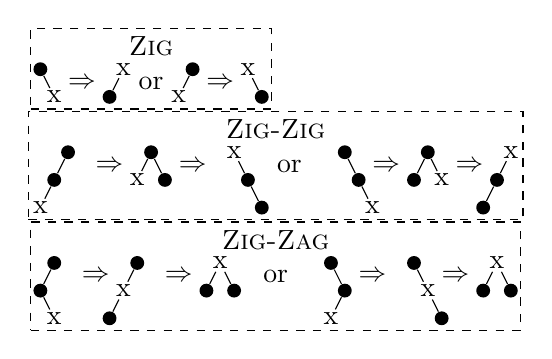
\begin{tikzpicture}[
              level distance= 10pt,
              every node/.style={circle, inner sep=0pt, minimum width=5pt}
        ]
            \begin{bscope}
                \begin{scope}[level/.style={sibling distance=10pt}]
                    \node[fill] {}
                      child [missing]
                      child {node {x}};
                \end{scope}
                
                \node [] at (15pt, -5pt) {$\Rightarrow$};
                
                \begin{scope}[level/.style={sibling distance=10pt}, xshift=30pt]
                    \node {x}
                      child {node[fill] {}}
                      child [missing];
                \end{scope}

                \node [] at (40pt, -5pt) {or};
                
                \begin{scope}[level/.style={sibling distance=10pt}, xshift=55]
                    \node[fill] {}
                      child {node {x}}
                      child [missing];
                \end{scope}
                
                \node [] at (65pt, -5pt) {$\Rightarrow$};
                
                \begin{scope}[level/.style={sibling distance=10pt}, xshift=75pt]
                    \node {x}
                      child [missing]
                      child {node[fill] {}};
                \end{scope}
                
                \node [yshift=5pt, inner sep=2pt, rectangle] at (bounding box \myscopelevel.north) {\sc Zig};
            \end{bscope}

            \begin{scope}[yshift=-30pt, xshift=10pt]
                \begin{bscope}
                    \begin{scope}
                        \begin{scope}[level/.style={sibling distance=10pt}]
                            \node[fill] {}
                                child {node[fill] {}
                                    child {node {x}}
                                    child [missing]
                                }
                                child [missing];
                        \end{scope}
                        
                        \node [] at (15pt, -5pt) {$\Rightarrow$};
                        
                        \begin{scope}[level/.style={sibling distance=10pt}, xshift=30pt]
                            \node[fill] {}
                                child {node {x}}
                                child {node[fill] {}};
                        \end{scope}
                        
                        \node [] at (45pt, -5pt) {$\Rightarrow$};
                        
                        \begin{scope}[level/.style={sibling distance=10pt}, xshift=60pt]
                            \node {x}
                                child [missing]
                                child {node[fill] {}
                                    child [missing]
                                    child {node[fill] {}}
                                };
                        \end{scope}
                    \end{scope}
                        
                    \node [] at (80pt, -5pt) {or};
                    
                    \begin{scope}[xshift=100pt]
                        \begin{scope}[level/.style={sibling distance=10pt}]
                            \node[fill] {}
                                child [missing]
                                child {node[fill] {}
                                    child [missing]
                                    child {node {x}}
                                };
                        \end{scope}
                        
                        \node [] at (15pt, -5pt) {$\Rightarrow$};
                        
                        \begin{scope}[level/.style={sibling distance=10pt}, xshift=30pt]
                            \node[fill] {}
                                child {node[fill] {}}
                                child {node {x}};
                        \end{scope}
                        
                        \node [] at (45pt, -5pt) {$\Rightarrow$};
                        
                        \begin{scope}[level/.style={sibling distance=10pt}, xshift=60pt]
                            \node {x}
                                child {node[fill] {}
                                    child {node[fill] {}}
                                    child [missing]
                                }
                                child [missing];
                        \end{scope}
                    \end{scope}
                    
                    \node [yshift=5pt, inner sep=2pt, rectangle] at (bounding box \myscopelevel.north) {\sc Zig-Zig};
                \end{bscope}
            \end{scope}

            \begin{scope}[yshift=-70pt, xshift=5pt]
                \begin{bscope}
                    \begin{scope}
                        \begin{scope}[level/.style={sibling distance=10pt}]
                            \node[fill] {}
                                child {node[fill] {}
                                    child [missing]
                                    child {node {x}}
                                }
                                child [missing];
                        \end{scope}
                        
                        \node [] at (15pt, -5pt) {$\Rightarrow$};
                        
                        \begin{scope}[level/.style={sibling distance=10pt}, xshift=30pt]
                            \node[fill] {}
                                child {node {x}
                                    child {node[fill] {}}
                                    child [missing]
                                }
                                child [missing];
                        \end{scope}
                        
                        \node [] at (45pt, -5pt) {$\Rightarrow$};
                        
                        \begin{scope}[level/.style={sibling distance=10pt}, xshift=60pt]
                            \node {x}
                                child {node[fill] {}}
                                child {node[fill] {}};
                        \end{scope}
                    \end{scope}
                        
                    \node [] at (80pt, -5pt) {or};
                    
                    \begin{scope}[xshift=100pt]
                        \begin{scope}[level/.style={sibling distance=10pt}]
                            \node[fill] {}
                                child [missing]
                                child {node[fill] {}
                                    child {node {x}}
                                    child [missing]
                                };
                        \end{scope}
                        
                        \node [] at (15pt, -5pt) {$\Rightarrow$};
                        
                        \begin{scope}[level/.style={sibling distance=10pt}, xshift=30pt]
                            \node[fill] {}
                                child [missing]
                                child {node {x}
                                    child [missing]
                                    child {node[fill] {}}
                                };
                        \end{scope}
                        
                        \node [] at (45pt, -5pt) {$\Rightarrow$};
                        
                        \begin{scope}[level/.style={sibling distance=10pt}, xshift=60pt]
                            \node {x}
                                child {node[fill] {}}
                                child {node[fill] {}};
                        \end{scope}
                    \end{scope}
                    
                    \node [yshift=5pt, inner sep=2pt, rectangle] at (bounding box \myscopelevel.north) {\sc Zig-Zag};
                \end{bscope}
            \end{scope}
        \end{tikzpicture}        

        Keep doing this until the node is at the top.



        \subsection{Search}
        Let $k$ be the target key we are searching for.
        
        Call \texttt{splay}($k$). The result is either
        \begin{enumerate}
            \item The key itself
            \item Its inorder successor
            \item Its inorder predecessor
        \end{enumerate}

        {\bf Average Case}: $\O(\log n)$
        
        {\bf Worst Case}: $\O(n)$



        \subsection{Insert}
        Let $k$ be the key to insert.

        Call \texttt{splay}($k$), one of two things can happen
        \begin{enumerate}
            \item $k$ is now at the root. If so, error
            \item $y$ is now at the root (the inorder pred/succ of $k$). Then let $k$ be the new root and attach $y$ as its child.
        \end{enumerate}

        {\bf Average Case}: $\O(\log n)$, {\bf Worst Case}: $\O(n)$



        \subsection{Delete}
        Let $k$ be the key to delete.

        Call \texttt{splay}($k$), one of two things can happen
        \begin{enumerate}
            \item $k$ is not at the root. If so, error
            \item $k$ is now at the root with left subtree $L$ and right subtree $R$.
            \begin{enumerate}
                \item If either $R$ or $L$ is empty, delete $x$ and set the non-empty sub-tree as the root.
                \item Otherwise, let $T$ be the non-empty subtree.
                \begin{enumerate}
                    \item Call $T$.\texttt{splay}($k$) to bring up inorder pred/succ $y$.
                    \item One of the subtrees of $y$ will be empty. Delete $k$ and set $y$ to be the new root.
                \end{enumerate}
            \end{enumerate}
        \end{enumerate}

        {\bf Average Case}: $\O(\log n)$, {\bf Worst Case}: $\O(n)$


        
        \section{Skip Lists}
        {\it A multi-lane linked list}.

        \subsection{Parameters}
        \begin{enumerate}
            \item  $L$: Maximum number of levels. Treated as constant
            \item $n$: Number of nodes
        \end{enumerate}

        \subsection{Probabilities}

        Let $0 < p < 1$ be the probability of adding a level.
        \begin{enumerate}
            \item Probability that at least one node reaches level $L \ge 0$ or more: $(1 - (1 - p^L))^n$
            \item Probability that at least one node reaches level $L \ge 0$ is bounded by $n p^L$
            \item Expected max level for $n$ nodes: $\Theta(\log_{1 / p} n)$
            \item Expected max level for $n$ nodes: $1 + \log_{1 / p} n$
            \item Expected number of levels: $2 + \log_{1 / p} n$
        \end{enumerate}



        \subsection{Insert}
        Let $x$ be the key to insert.

        \begin{enumerate}
            \item Go to $x$.
            \begin{enumerate}[label=\roman*.]
                \item Take the fastest lane (the highest) and stop at the largest key less than $x$. Record all pointers as you go
                \item Go down by one lane and repeat step 1, until you are at the lowest lane.
            \end{enumerate}
            \item Insert $x$. % \TODO{} explain how specifically
            \begin{enumerate}[label=\roman*.]
                \item Flip a probability $p$ coin until you get $0$, or you've flipped it $L$ times.
                Add as many lanes to $x$ as the number of times you've flipped it.
                
                \item Add the recorded pointers to $x$.

                \item update the previous pointers to now point to $x$.
            \end{enumerate}
        \end{enumerate}

        {\bf Average Case}: $\O(\log n)$, {\bf Worst Case}: $\O(n)$

        

        \subsection{Delete}

        % \TODO{} Elaborate
        \begin{enumerate}
            \item Go to $x$, using the same technique as above, still recording pointers as you go.
            \item Record all pointers of $x$.
            \item Delete $x$.
            \item Update all pointers pointing to $x$ to now point to where $x$ was pointing to.
        \end{enumerate}

        {\bf Note}: Fixing the number of pointers is $\O(1)$

        {\bf Average Case}: $\O(\log n)$, {\bf Worst Case}: $\O(n)$


        
        \section{KD-Trees}

        \subsection{Height}
        \begin{enumerate}
            \item Best Case: $\O(\log n)$
            \item Average Case: $\O(\sqrt n)$
            \item Worst Case: $\O(n)$
        \end{enumerate}

        \subsection{Search}
        \begin{enumerate}
            \item Root splits on first dimension axis $\alpha$, $x$ for 2D or 3D.
            \item In case of ties for axis $\alpha$, go right.
            \item Each layer splits by the next axis.
            \begin{enumerate}[label=\roman*.]
                \item 2D: $x \to y \to x \to \cdots$
                \item 3D: $x \to y \to z \to x \to \cdots$
            \end{enumerate}
        \end{enumerate}

        {\bf Worst Case}: $\O(n)$ since we don't re-balance at all.

        \subsection{Insert}
        Let $n$ be the node to insert.
        \begin{enumerate}
            \item Go through tree as if searching for $n$.
            \item Insert as BST.
        \end{enumerate}

        {\bf Worst Case}: $\O(n)$ since we don't re-balance at all.

        \subsection{Delete}
        Let $n$ be the node to delete.
        \begin{enumerate}
            \item Search for $n$ in the tree.
            \item If $n$ is a leaf, delete it and you're done.
            
            \item If $n$ is not a leaf, say $n$ splits by $\alpha$. Replace $n$ with the node $n'$ with minimum $\alpha$ in the {\it right subtree} of $n$.
            \item If $n$ has no right subtree, it {\it must} have a left subtree. Replace $n$ with the node $n'$ in the left subtree with minimum $\alpha$. Update the left subtree to become the right subtree.
            
            {\bf Note}: $n'$ might not be a leaf, $n'$ might not split by $\alpha$. That's fine.
            
            \item Recursively call \texttt{delete($n'$)}.
        \end{enumerate}

        {\bf Worst Case}: $\O(n)$ since we don't re-balance at all.

        \section{Ext. KD-Trees}

        \subsection{Parameters}
        \begin{enumerate}
            \item $m$: The maximum leaf size.
        \end{enumerate}

        \subsection{Split Method}
        \begin{enumerate}
            \item {\bf Cycle Split}: Split by $x \to y \to z \to x \to \cdots$
            \item {\bf Spread Split}: Split by axis $\alpha$ with largest spread.
        \end{enumerate}
        
        \subsection{Search}
        Let $n$ be the node to search.
        \begin{enumerate}
            \item Follow splitting nodes down the tree.
            \item If a splitting node has same axis value as $n$, check both subtrees.
        \end{enumerate}

        \subsection{Insert}
        Let $n$ be the node to insert.
        \begin{enumerate}
            \item Follow splitting nodes down the tree.
            \item If a splitting node has same axis value as $n$, {\bf only go right}.
            \item Insert into leaf.
            \begin{enumerate}[label=\roman*.]
                \item If leaf size is less than or equal to $m$, done.
                \item If leaf size is more than $m$, split by Split Method.
            \end{enumerate}
        \end{enumerate}

        \subsection{Delete}
        Let $n$ be the node to delete.
        \begin{enumerate}
            \item Follow splitting nodes down the tree as if searching for $n$.
            \item If leaf becomes empty, delete splitting node and merge with sibling.
        \end{enumerate}

        \subsection{KNN}

        Let $P$ be the coordinate, let $k$ be the number of neighbors, let $L = \texttt{[]}$ be the list of nearest neighbors, let $d^* = \max_{p \in L}$ \texttt{dist($p$, $P$)}.

        % \subsubsection{Distance}

        % \begin{enumerate}
        %     \item {\bf Points}: $\texttt{dist}(p_1, p_2) = d^2 = (p_1.x - p_2.x)^2 + (p_1.y - p_2.y)^2 + (p_1.x - p_2.z)^2$
        %     \item {\bf Bounding Box}: $\texttt{dist}(p_1, b) = d^2 = (p_1.x - p_2.x)^2 + (p_1.y - p_2.y)^2 + (p_1.x - p_2.z)^2$ \TODO{}
        % \end{enumerate}
        

        \begin{enumerate}
            \item If we are at a leaf, add every node to $L$, sort by distance from $P$, only keep first $k$.
            \item If we are at a splitting node
            \begin{enumerate}
                \item If the list is not full, recurse to child with closest bounding box, if tied, prefer left. When checking both subtrees $L$ then $R$, check \texttt{dist}($d^*$, $R$) again before checking $R$, as $d^*$ could have changed from $L$.
                \item If the list is full, compute $d^*$.
                \begin{enumerate}
                    \item If either subtree's bounding box is closer to $P$ than $d^*$, check it. In case of ties, check left first. When checking both subtrees $L$ then $R$, check \texttt{dist}($d^*$, $R$) again before checking $R$, as $d^*$ could have changed from $L$.
                \end{enumerate}
            \end{enumerate}
        \end{enumerate}

        \section{Tries}
        {\it Only one character per branch}.

        \subsection{Search}
        Follow the prefixes until you reach a $\$$ node.

        \subsection{Insert}
        Follow the tree until we fall out. Then build out a new branch of the tree if necessary.

        \subsection{Delete}
        Follow the path to the leaf, then travel back to the furthest ancestor which has more than one (non-null) child and remove the corresponding branch.
        
        \section{Compressed Tries}

        \subsection{Insert}
        Let $s$ be the string to insert.
        \begin{enumerate}
            \item If a prefix of $s$ fully matches a branch, follow it and recurse with the rest of $s$. 
            \item If no prefix of $s$ matches any branch, make a new branch.
            \item If a prefix of $s$ partially matches a branch $b$, split $b$ by the largest shared component, add a branch with the rest of $s$ and add a branch with the rest of $b$ with its children.
        \end{enumerate}



        \subsection{Delete}
        Let $s$ be the string to delete.
        \begin{enumerate}
            \item Remove the final branch corresponding to $s$.
            \item If the parent of that branch only has one child, merge the two edges into one.
        \end{enumerate}


        \subsection{Height Bounds}
        Let $h$ be the height of the trie.
        \begin{enumerate}
            \item $h \le 1 + \text{max word length}$. Good if you have {\it many}, {\it short} words.
            \item $h \le 1 + n$. Good if you have {\it few}, {\it long} words.
        \end{enumerate}
        
        
        \section{Hash Functions}

        \subsection{Parameters}
        \begin{enumerate}
            \item $h$: A hash function.
            \item $n$: Number of keys inserted.
            \item $m$: Size of the hash table.
            \item $\lambda = n / m$: Load factor of the hash table.
        \end{enumerate}

        \subsection{Addressing}
        \begin{enumerate}
            \item {\bf Closed Addressing}: Entries of the hash table point to a data structure.
            \item {\bf Open Addressing}: Keys are stored directly in the hash table.
        \end{enumerate}

        \subsection{Rebuilding}
        Rebuild after insert, if $\lambda > \lambda_\text{max}$. The new size
        of the hash table is $m' = \ce{2n / (\lambda_\text{min} + \lambda_\text{max})}$, 
        where $0 \le \lambda_\text{min}, \lambda_\text{max} \le 1$.

        We also rebuild after a delete takes us out of the acceptable range:  $\lambda <
        \lambda_\text{min}$. If we delete and we were already below acceptable range,
        we don't rebuild.

        \subsection{Probing}
        {\it Only occurs with Open Addressing}.

        Method by which we find an open spot in the Hash Table if there is a collision.
        Linear Probing hits every slot, quadratic probing hits at least $\floor{\frac{m}{2}}$ slots if $m$ is prime.
        \section{Bloom Filters}

        \subsection{Parameters}
        \begin{enumerate}
            \item $B$: The bit array.
            \item $k$: Number of hash functions.
            \item $m$: Size of the bloom filter.
            \item $n$: Number of inserts.
        \end{enumerate}

        \subsection{Insert}
        Let $s$ be the inputted value. For each hash function $h_k$, set $B[h_k(s)] = 1$.

        {\bf Time Complexity}: $\Theta(1)$, $k$ is a constant.

        \subsection{Probabilities}

        Probability of false positive: $p = \left(1 - \left(1 - \frac{1}{m}\right)^{kn}\right)^k$.

        \subsection{Deletion}
        No deletion since it could introduce false negatives.

        \subsection{Rebuilding}

        Rebuild as with hash function.


        
        
        \section{Disjoint Set Data Structures}
            {\it A forest where every node points to its parent. Roots point to themselves.}

            \subsection{\texttt{find\_rep}}
            For a node $v$, \texttt{find\_rep}($v$) is itself if $v$\texttt{.parent = $v$}.
            Otherwise, \texttt{find\_rep($v$) = find\_rep($v$.parent)}.

            If \texttt{find\_rep($v$) = find\_rep($u$)}, then $v$ and $u$ are in the same tree.
            
            \subsection{Path Compression}
            For a node $n$, let $r$ be the root pointer for the tree. When \texttt{find\_rep}($n$) is called, every node on the path back from $n$ to $r$ has its parent pointer updated to $r$.
            
            % Whenever you follow these pointers, rewire every pointer you cross to go directly to the root.

            \subsection{Weighted Union}
            For two trees $T_1$ and $T_2$, with $|T_1| < |T_2|$, set \texttt{parent($r_1$) = $r_2$} where $r_i$ is the root of $T_i$.

            % \textbf{Weighted Union} - Wire the tree with fewer nodes into the tree with more nodes (this is a heuristic, we would really want height, but node count is easier to track)

            {\bf Time Complexity}: $\O(\alpha(n))$ where $\alpha(n)$ is the Inverse Ackermann function, $\alpha(n) < 5$ for any $n$ that can fit.
    \end{multicols*}
\end{document}
